%%%%%%%%%%%%%%%%%%%%%%%%%%%%%%%%%%%%%%%%%%%%%%%%%%%%%%%%%%%%%
%% Prozedural/Funktional programmieren
%%%%%%%%%%%%%%%%%%%%%%%%%%%%%%%%%%%%%%%%%%%%%%%%%%%%%%%%%%%%%
\chapter{Aufgabe 4}
\label{sec:aufgabe4}

\subsection*{a)}
Vervollständigen Sie das folgende Java-Programm, indem Sie die aufgerufenen Klassenmethoden ergänzen.
Was an dem Java-Programm ist eindeutig prozeduraler Stil?
\newline
\begin{code}[language=java, caption={Vorgabe}, label={lst:Aufgabe4a}]
import java.nio.file.Files;
import java.nio.file.Paths;
import java.io.BufferedReader;
import java.io.IOException;

import java.util.LinkedList;
import java.util.List;

public final class Procedural {
    private Procedural() { }

    private static final int MIN_LENGTH = 20;

    public static void main(String[] args) throws IOException {
        var input = Files.newBufferedReader(Paths.get(args[0]));
        var lines = new LinkedList<String>();

        long start = System.nanoTime();

        readLines(input, lines);
        removeEmptyLines(lines);
        removeShortLines(lines);
        int n = totalLineLengths(lines);

        long stop = System.nanoTime();

        System.out.printf("result = %d (%d microsec)%n", n, (stop - start) / 1000);
    }

    private static void readLines(BufferedReader input, List<String> lines) throws IOException {
        String line;
        while ((line = input.readLine()) != null) {
            lines.add(line);
        }
    }

    // TODO: Klassenmethoden readLines, removeEmptyLines, removeShortLines, totalLineLengths
}
\end{code}
\newline

\subsection*{a - Lösung}
\newline
\begin{code}[language=java, caption={Prozedurale Methoden}, label={lst:Aufgabe4a}]
    private static void removeEmptyLines(List<String> lines) {
        for (var it = lines.iterator(); it.hasNext(); ) {
            if (it.next().isEmpty()) {
                it.remove();
            }
        }
    }

    private static void removeShortLines(List<String> lines) {
        for (var it = lines.iterator(); it.hasNext(); ) {
            if (it.next().length() < MIN_LENGTH) {
                it.remove();
            }
        }
    }

    private static int totalLineLengths(List<String> lines) {
        int n = 0;
        for (var it = lines.iterator(); it.hasNext(); ) {
            n += it.next().length();
        }
        return n;
    }
\end{code}
\newline
Die Aufrufe der Klassenmethoden sind im Prozeduralen Stil.
Typisch dafür ist die beschreibende Programmierung, bei der die Methoden in der Reihenfolge aufgerufen werden, wie man es auch beschreiben würde.
Methoden geben dann typischerweise keinen Wert zurück, sondern verändern den Zustand der Objekte, die sie als Parameter erhalten.
\newline

\subsection*{b)}
Stellen Sie das Programm aus 4a mit Hilfe von \textit{java.util.streams} und Lambdas auf einen funktionalen Stil um.
Ihr Programm darf nach der Umstellung keine Schleifen, Verzweigungen und Seiteneffekte mehr enthalten.
\newline
\newline
\subsection*{b - Lösung}
\newline
\begin{code}[language=java, caption={Funktionale Methoden}, label={lst:Aufgabe4b}]
public final class ProceduralFunctional {
    private ProceduralFunctional() { }

    private static final int MIN_LENGTH = 20;

    public static void main(String[] args) throws IOException {
        var input = Files.newBufferedReader(Paths.get(args[0]));

        long start = System.nanoTime();

        int n = input.lines()
                .filter(s -> !s.isEmpty())
                .filter(s -> s.length() >= MIN_LENGTH)
                .mapToInt(String::length)
                .sum();

        long stop = System.nanoTime();

        System.out.printf("result = %d (%d microsec)%n", n, (stop - start) / 1000);
    }
}
\end{code}
\newline
Die vorherigen Klassenmethoden wurden durch funktionalen Stil ersetzt.
Zu erst wird ein Stream aus den Zeilen der Datei erstellt,
auf welchen dann die Filteroperationen angewendet werden.
Die Filteroperationen sind in der Reihenfolge aufgelistet, wie sie auch in der Beschreibung des Programms stehen
- Könnten aber auch zusammengefasst werden.
Die Filteroperationen geben einen neuen Stream zurück, auf welchem dann die nächste Operation angewendet wird.
Gefilterte Zeilen werden auf die Länge gemappt und anschließend wird die Gesamtsumme gebildet,
 so wie es auch der prozedurale Stil getan hat.
\newline

\subsection*{c)}
Vergleichen Sie die Laufzeiten der Programme aus 4a und 4b.
\newline
\subsection*{c - Lösung}
\newline
\begin{code}[language=text, caption={input.txt}, label={lst:Aufgabe4c}]
Lorem ipsum dolor sit amet, consectetur adipiscing elit.
Sed et metus aliquam, hendrerit metus vel, rhoncus dolor.
Nulla facilisi. Nullam a sapien libero.
Morbi in erat sit amet enim sagittis semper.
Fusce at leo vitae ligula malesuada luctus.
Curabitur sed lectus in nisi vulputate sodales. Nulla facilisi.
Morbi auctor, dolor nec ultricies tincidunt, justo felis pharetra mauris, a lacinia quam arcu et nisl.
Suspendisse potenti. Morbi euismod augue lacus, vitae faucibus libero bibendum non.
Nullam nec augue ut mi cursus hendrerit. In hac habitasse platea dictumst.

Nullam ut neque ligula. Aliquam erat volutpat. Nulla facilisi.
Duis nec urna sed lacus vestibulum viverra.
Donec nec ante sit amet erat ultrices iaculis.
Sed id tortor quis turpis pellentesque egestas.
Pellentesque.

\end{code}
\newline
\begin{figure}[h]
	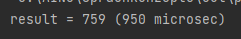
\includegraphics[width=\textwidth]{media/Aufgabe4c_procedural}
	\caption{Prozedural}
	\label{img:Aufgabe4c_procedural}
\end{figure}
\begin{figure}[h]
	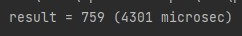
\includegraphics[width=\textwidth]{media/Aufgabe4c_functional}
	\caption{Funktional}
	\label{img:Aufgabe4c_functional}
\end{figure}
\newline
Wie erwartet ist der funktionale Stil deutlich langsamer als der prozedurale Stil.
Dies ist zurückzuführen auf die Tatsache, dass der funktionale Stil mit \textit{Streams}, intern mit Rekursion arbeitet.
Im prozeduralen Stil werden die Operationen in einfachen Schleifen ausgeführt, wodurch die Laufzeit kurz bleibt.
\newline
